% Rule structure figure for the manuscript. Build: pdflatex rule_structure.tex
\documentclass[border=4pt]{standalone}
\usepackage[T1]{fontenc}
\usepackage{lmodern}
\usepackage{amsmath}
\usepackage{tikz}
\usetikzlibrary{positioning,arrows.meta,calc}
\renewcommand{\familydefault}{\sfdefault}
\begin{document}
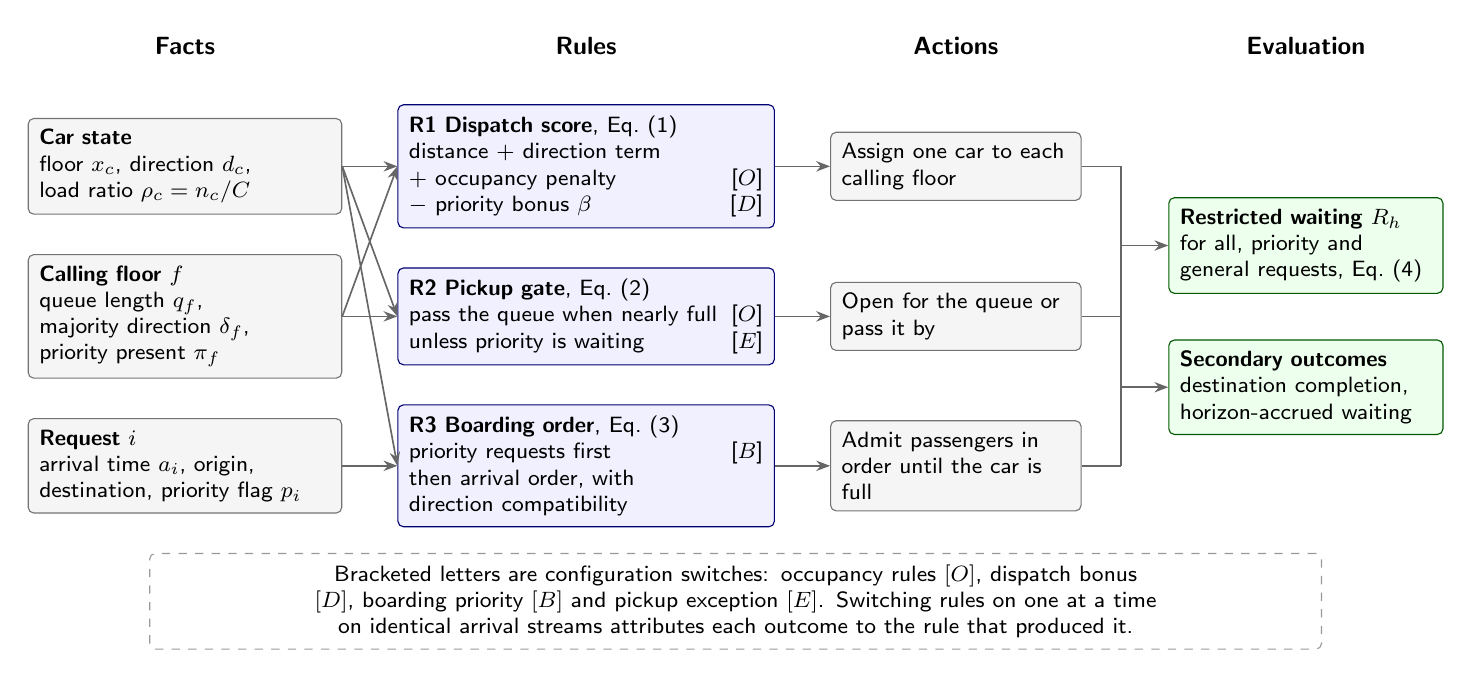
\begin{tikzpicture}[
  font=\sffamily\footnotesize,
  box/.style={draw=black!55, rounded corners=2pt, align=left, inner sep=4pt, text width=#1},
  box/.default=3.7cm,
  fact/.style={box, fill=black!4},
  rule/.style={box=4.5cm, fill=blue!6, draw=blue!45!black},
  act/.style={box=2.9cm, fill=black!4},
  outc/.style={box=3.2cm, fill=green!7, draw=green!35!black},
  head/.style={font=\sffamily\small\bfseries, anchor=south},
  arr/.style={-{Stealth[length=5pt]}, draw=black!60, line width=.6pt},
  ln/.style={draw=black!60, line width=.6pt},
  node distance=5mm and 7mm]

% Facts
\node[fact] (car) {\textbf{Car state}\\ floor $x_c$, direction $d_c$,\\ load ratio $\rho_c=n_c/C$};
\node[fact, below=of car] (queue) {\textbf{Calling floor} $f$\\ queue length $q_f$,\\ majority direction $\delta_f$,\\ priority present $\pi_f$};
\node[fact, below=of queue] (req) {\textbf{Request} $i$\\ arrival time $a_i$, origin,\\ destination, priority flag $p_i$};

% Rules
\node[rule, right=of car] (r1) {\textbf{R1 Dispatch score}, Eq.~(1)\\ distance + direction term\\ + occupancy penalty \hfill[$O$]\\ $-$ priority bonus $\beta$ \hfill[$D$]};
\node[rule, right=of queue] (r2) {\textbf{R2 Pickup gate}, Eq.~(2)\\ pass the queue when nearly full \hfill[$O$]\\ unless priority is waiting \hfill[$E$]};
\node[rule, right=of req] (r3) {\textbf{R3 Boarding order}, Eq.~(3)\\ priority requests first \hfill[$B$]\\ then arrival order, with\\ direction compatibility};

% Actions
\node[act, right=of r1] (a1) {Assign one car to each calling floor};
\node[act, right=of r2] (a2) {Open for the queue or pass it by};
\node[act, right=of r3] (a3) {Admit passengers in order until the car is full};

% Outcomes
\coordinate (bus) at ($(a2.east)+(5mm,0)$);
\node[outc, anchor=west] (o1) at ($(bus)+(6mm,9mm)$) {\textbf{Restricted waiting} $R_h$\\ for all, priority and\\ general requests, Eq.~(4)};
\node[outc, anchor=west] (o2) at ($(bus)+(6mm,-9mm)$) {\textbf{Secondary outcomes}\\ destination completion,\\ horizon-accrued waiting};

% Column headings
\node[head] at (car.north |- 0,1.3) {Facts};
\node[head] at (r1.north |- 0,1.3) {Rules};
\node[head] at (a1.north |- 0,1.3) {Actions};
\node[head] at (o1.north |- 0,1.3) {Evaluation};

% Fact-to-rule links
\draw[arr] (car.east) -- (r1.west);
\draw[arr] (car.east) -- (r2.west);
\draw[arr] (car.east) -- (r3.west);
\draw[arr] (queue.east) -- (r1.west);
\draw[arr] (queue.east) -- (r2.west);
\draw[arr] (req.east) -- (r3.west);
% Rule-to-action links
\draw[arr] (r1) -- (a1);
\draw[arr] (r2) -- (a2);
\draw[arr] (r3) -- (a3);
% Action-to-outcome links via a collector
\draw[ln] (a1.east) -- (bus |- a1.east);
\draw[ln] (a2.east) -- (bus);
\draw[ln] (a3.east) -- (bus |- a3.east);
\draw[ln] (bus |- a1.east) -- (bus |- a3.east);
\draw[arr] (bus |- o1.west) -- (o1.west);
\draw[arr] (bus |- o2.west) -- (o2.west);

% Switch legend, centred under the diagram
\node[draw=black!40, dashed, rounded corners=2pt, align=center, inner sep=4pt,
      text width=14.6cm, anchor=north] (legend)
  at ($(car.west |- req.south)!0.5!(o1.east |- req.south) + (0,-5mm)$)
  {Bracketed letters are configuration switches: occupancy rules $[O]$, dispatch bonus $[D]$, boarding priority $[B]$ and pickup exception $[E]$.
   Switching rules on one at a time on identical arrival streams attributes each outcome to the rule that produced it.};
\end{tikzpicture}
\end{document}
